\chapter{Implementation}

%The implementation should discuss any issues you encountered as you tried to implement your design. During the work, you might have found that elements of your design were unnecessary or overly complex; perhaps third-party libraries were available that simplified some of the functions that you intended to implement. If things were easier in some areas, then how did you adapt your project to take account of your findings?
%
%It is more likely that things were more complex than you first thought. In particular, were there any problems or difficulties that you found during implementation that you had to address? Did such problems simply delay you or were they more significant?
%
%You can conclude this section by reviewing the end of the implementation stage against the planned requirements. 

\section{Code Implementation \& Third-Party libraries}
As seen below the Website and Discord bot have been split up into two separate sections because during implementation I decided to make the systems separate. This helps with code maintainability, readability and allows the administrator who sets up this project to deploy the website and bot services on different containers or networks. For more information of third party libraries please see appendix A.

\subsection{Website Building and Final Design}
To create and run the website I've used a set of different libraries to perform certain tasks. Firstly I've used the Apache2 \cite{apache2} web hosting framework to host the website along with the library libapache2-mod-auth-openidc to reroute all incoming traffic to OpenID Connect \cite{OpenID} for user authentication. On top of these I have used the linux tool certbot \cite{certbot} to create a Let's Encrypt certificate for the website to enable HTTPS. 

As discussed previously in this document in section \ref{sec1:Research} there were many libraries that were considered when deciding on the website framework. Django \cite{Django} was the framework of choice and it is open-source and free to use on personal projects. It is also very useful as it generates the majority of the code required to create and run a website so most of the code used will be picked up by the system for UAP. Apart from the general template I created a "Django Application" called login that contains the files and code which is used to run the website. I can confirm that the folder, login, is all my own code and shouldn't fall under UAP.

The website pages also use a third party library called bootstrap \cite{bootstrap} that is used to generate responsive mobile-first CSS for the website. The final design of the website ended up being very similar to that of the mockups I made in section \ref{sec2:ui} and included below are some images from the final website.

\textbf{Note}: The navigation bars in the images below are smaller than the mockups due to the change in screen size. These images were taken on a 27inch monitor whereas the mockups were made for a 15inch monitor.

\begin{figure}[H]
	\centering
	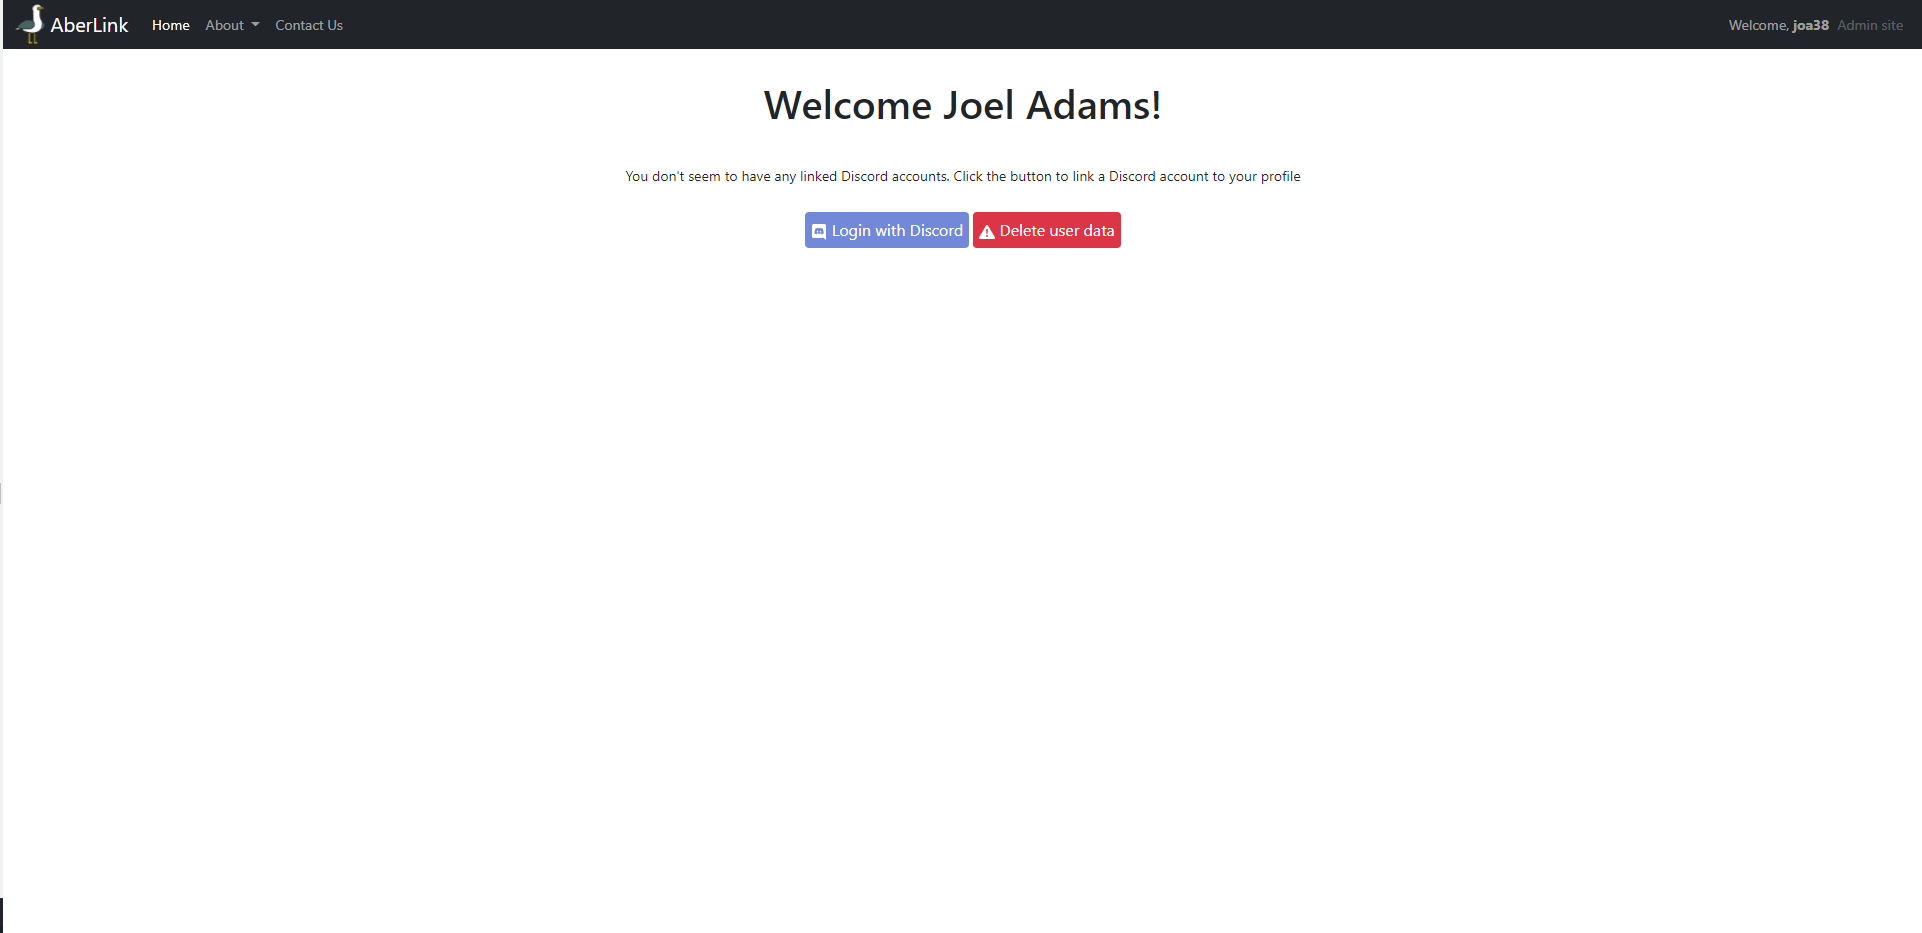
\includegraphics[width=1\linewidth]{Figures/website-acc-0.png}
	\caption{Final website with 0 linked Discord accounts}
	\label{fig:final-web-acc-0}
\end{figure}

\begin{figure}[H]
	\centering
	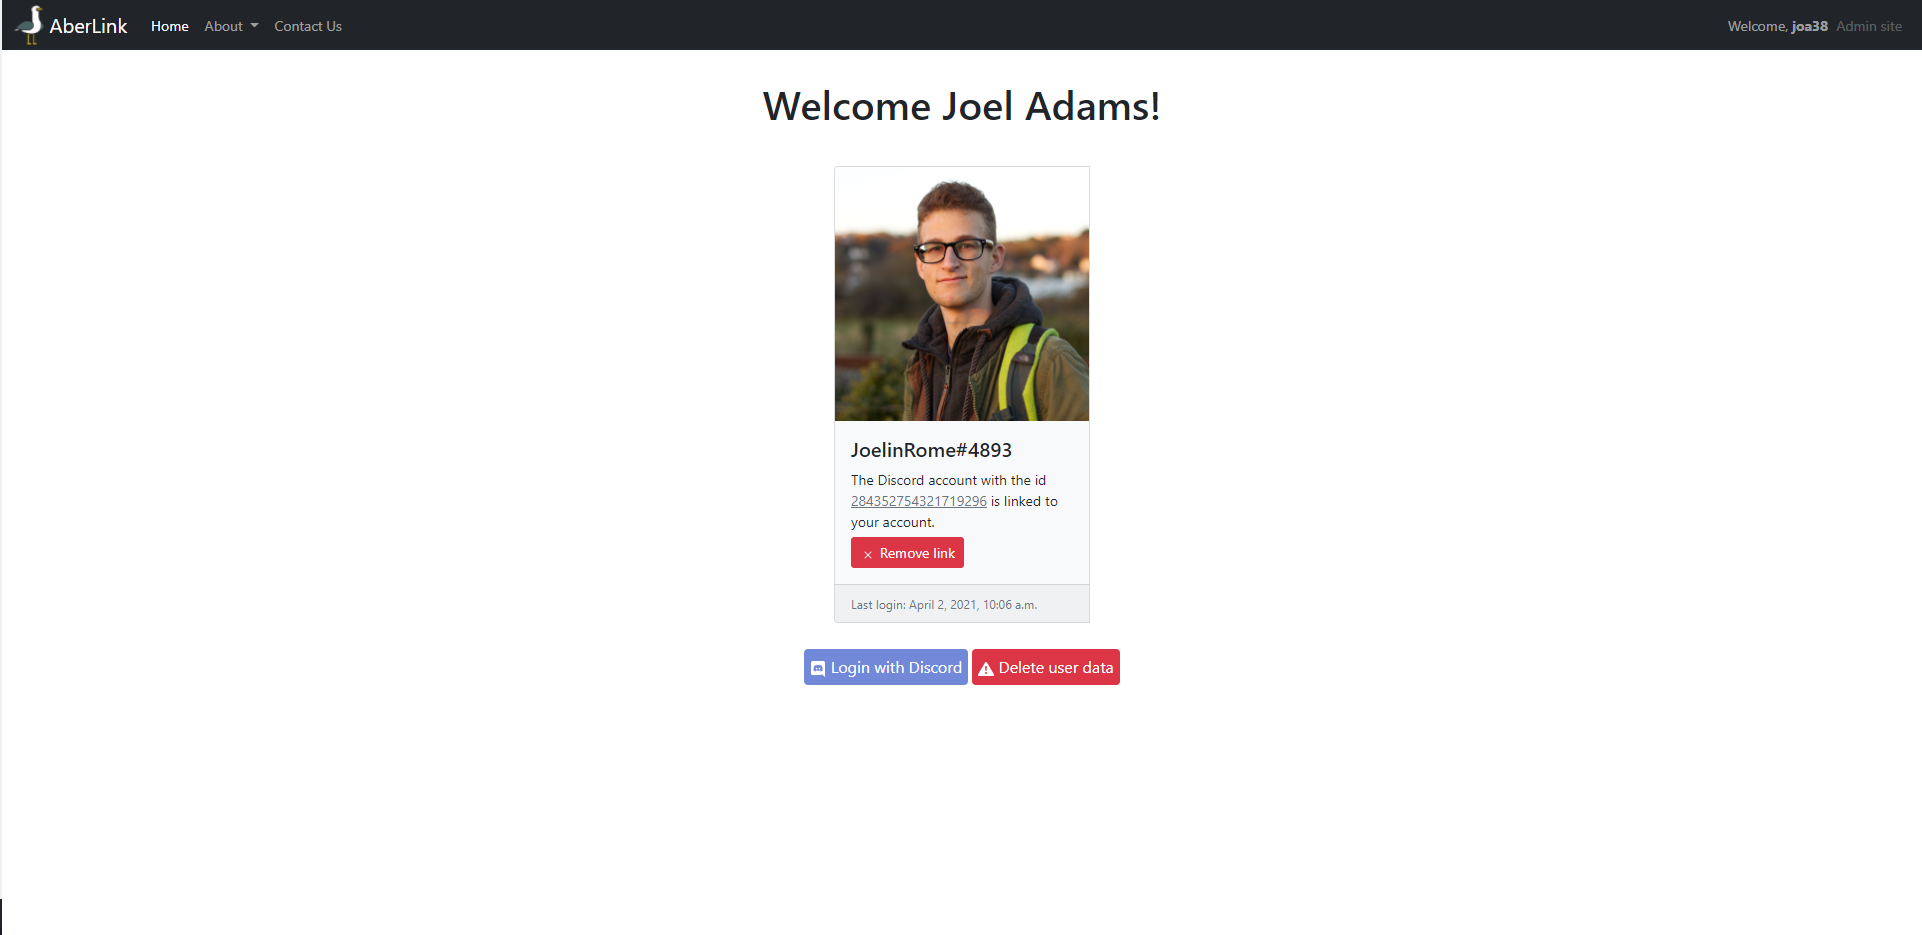
\includegraphics[width=1\linewidth]{Figures/website-acc-1.png}
	\caption{Final website with 1 linked Discord accounts}
	\label{fig:final-web-acc-1}
\end{figure}

\begin{figure}[H]
	\centering
	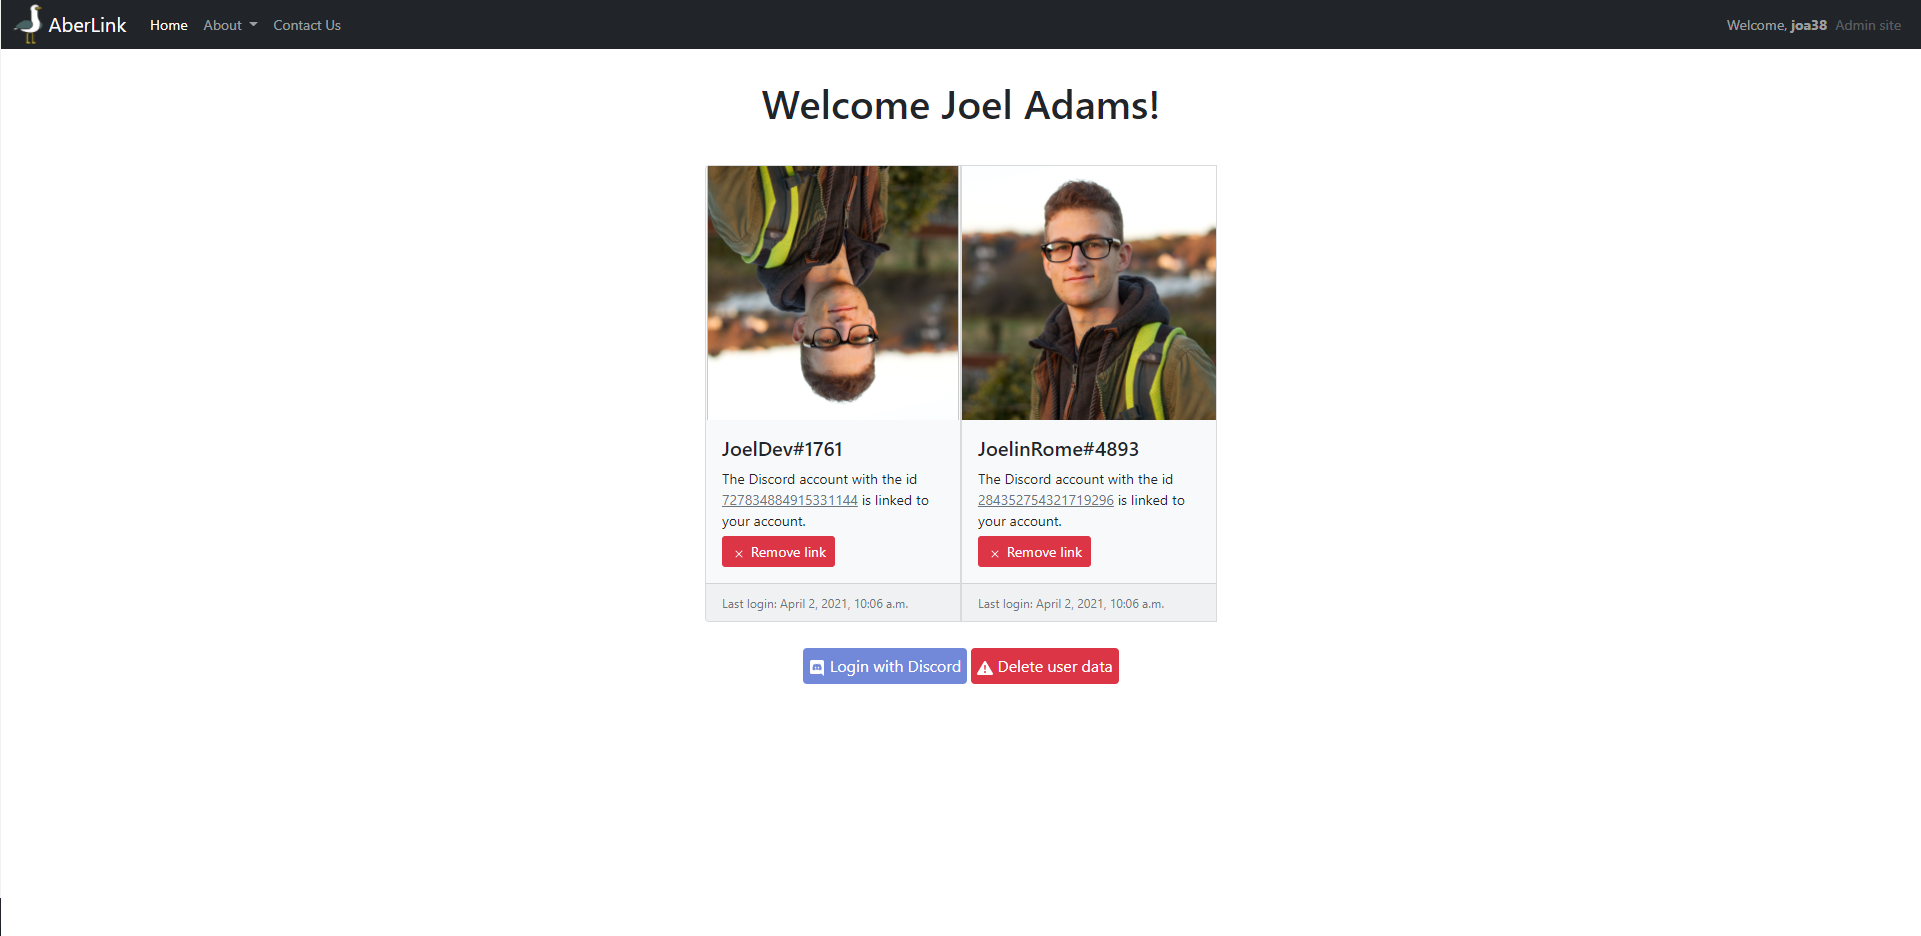
\includegraphics[width=1\linewidth]{Figures/website-acc-2.png}
	\caption{Final website with 2 linked Discord accounts}
	\label{fig:final-web-acc-2}
\end{figure}

\begin{figure}[H]
	\centering
	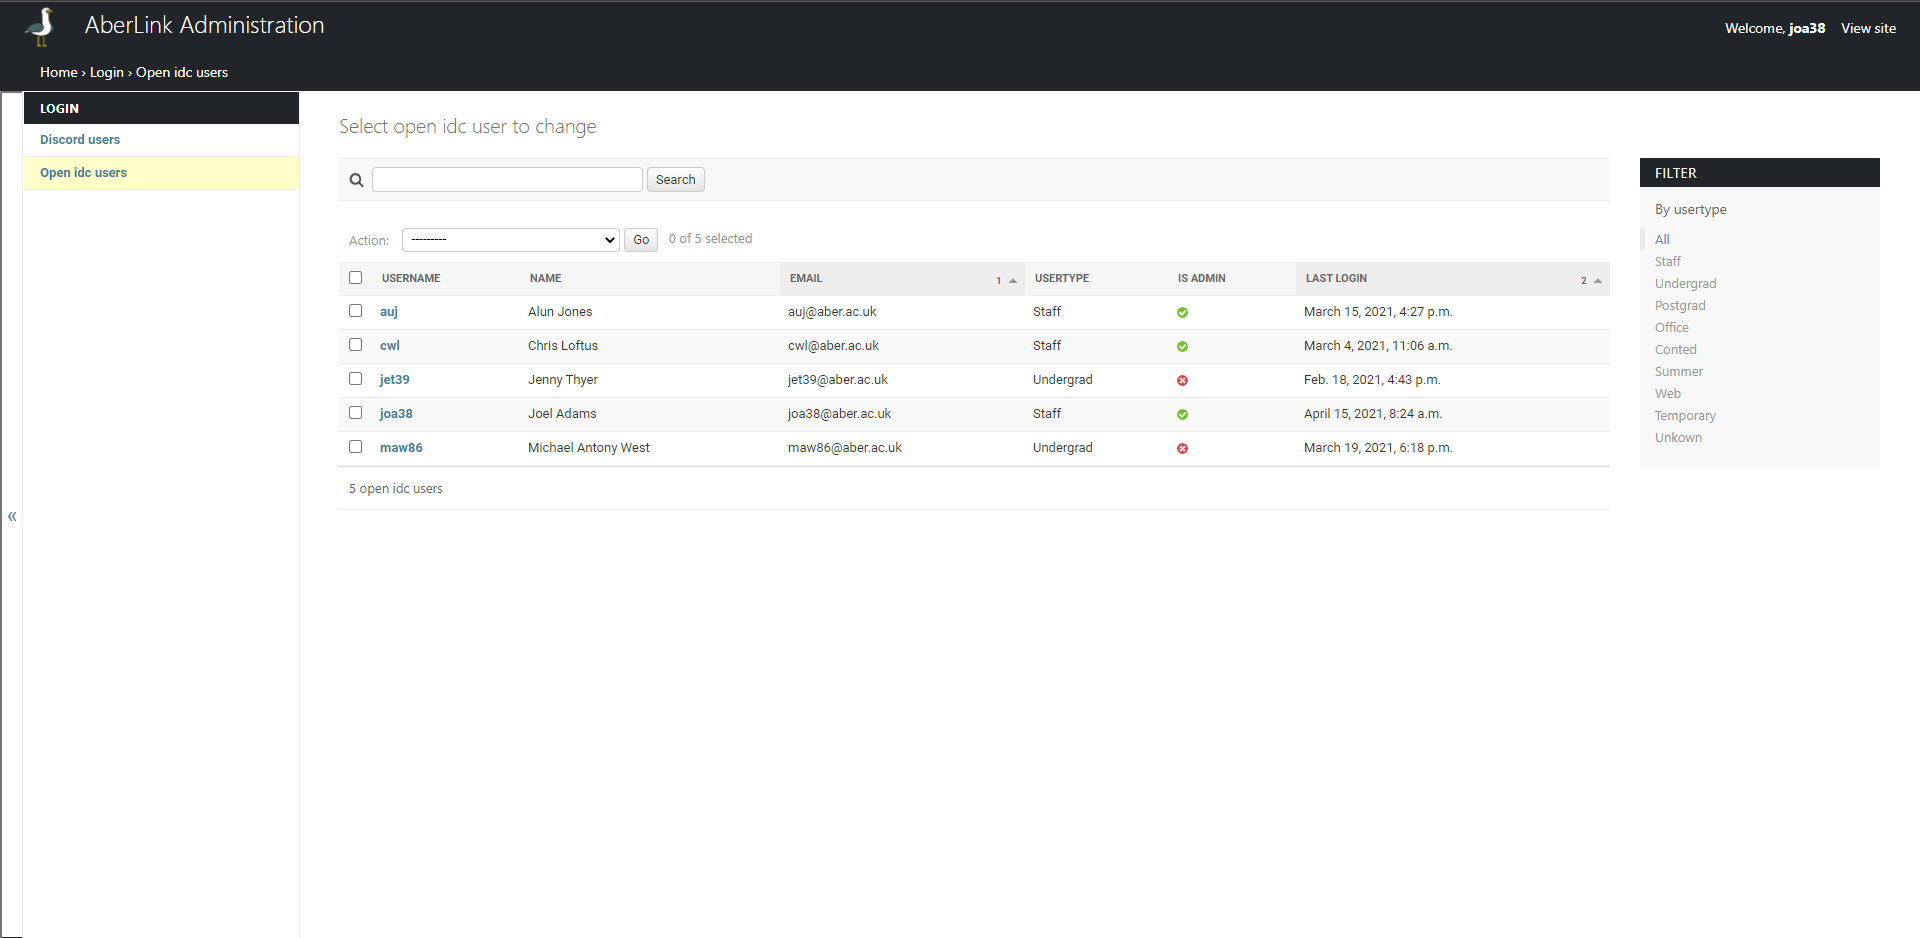
\includegraphics[width=1\linewidth]{Figures/website-admin-openidc.png}
	\caption{Final website Admin page for Aber accounts}
	\label{fig:final-web-admin-openidc}
\end{figure}

\begin{figure}[H]
	\centering
	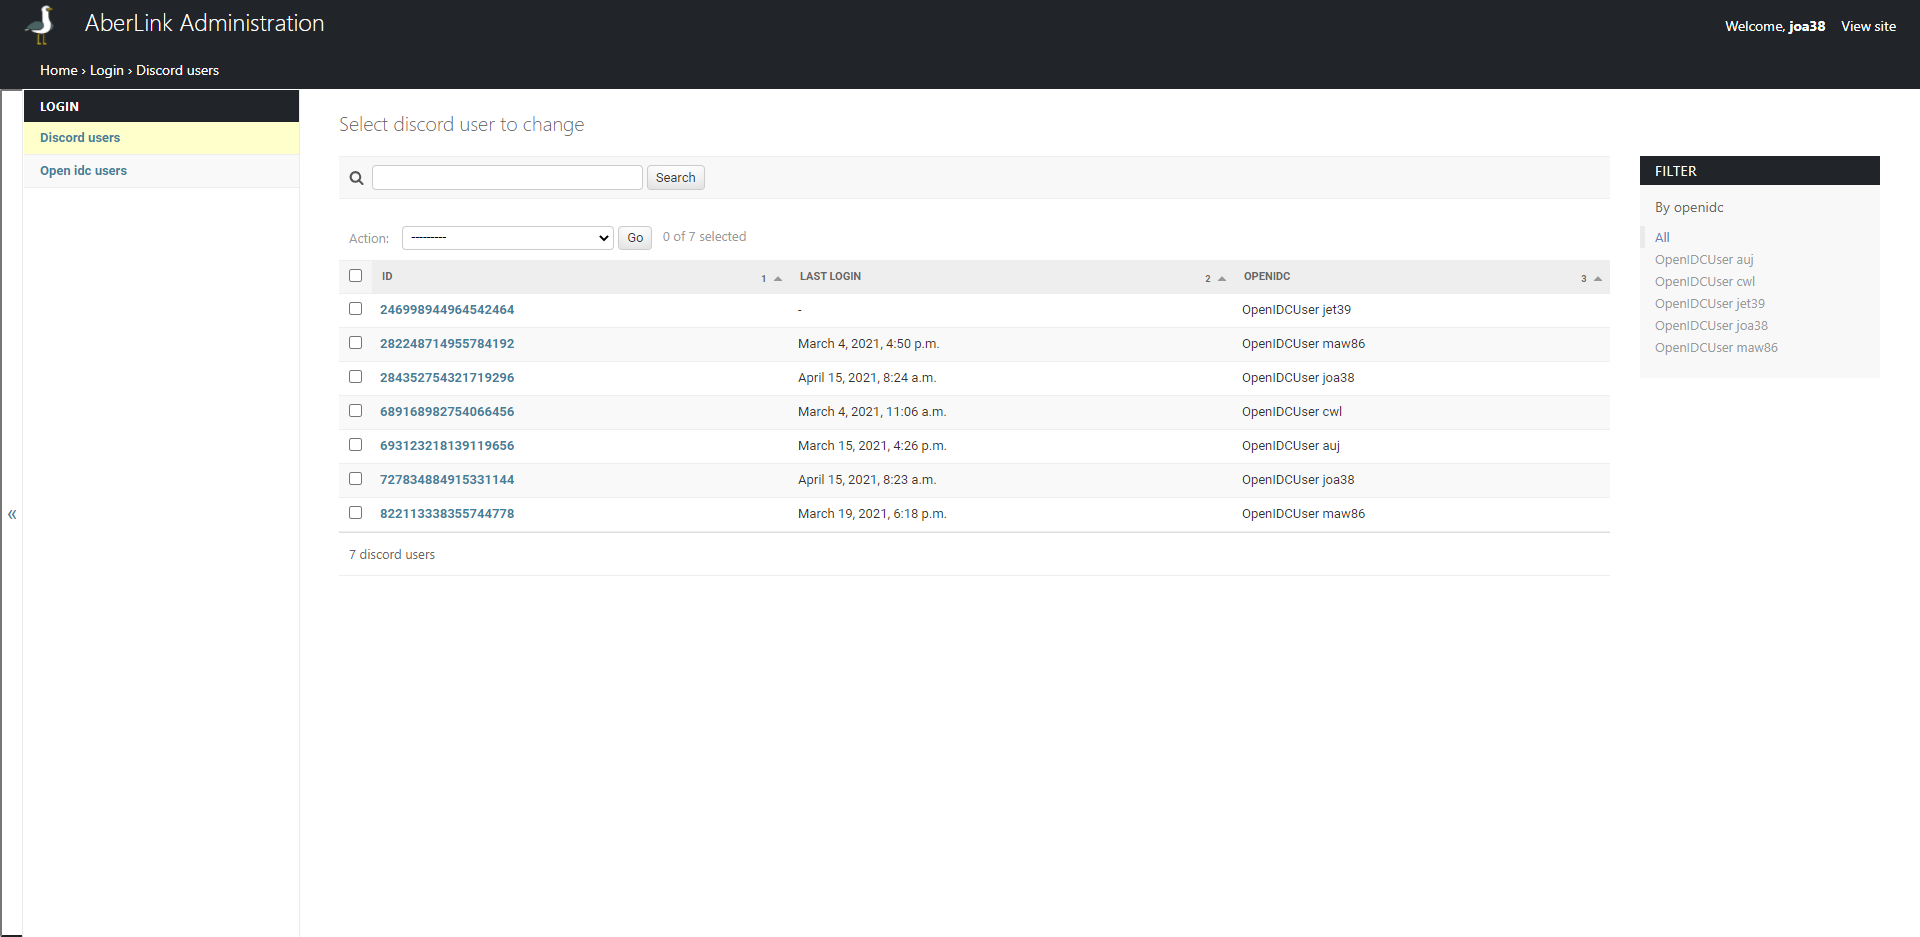
\includegraphics[width=1\linewidth]{Figures/website-admin-discord.png}
	\caption{Final website Admin page for Discord accounts}
	\label{fig:final-web-admin-dis}
\end{figure}

\subsection{Discord Bot}
The Discord bot (AberLink) implementation is exactly as described in the section \ref{sec2:discord} of the design. AberLink uses the Python library Discord.py \cite{discord.py} to make calls to and from the Discord API and to interact with the database it uses the Python library Psycopg2 \cite{psycopg2}. Both of these pieces of software are open-source and free to use in personal projects. 

\subsection{Database}\label{sec3:database}
The Database implementation was relatively straight forward as Django \cite{Django} generates all of the required tables for the project to function once you define the models. I've included the model used to generate OpenID Connect \cite{OpenID} aber user model below. In this figure you can see that there are two classes; OpenIDCUserManager to create a new database object and OpenIDCUser to make the database model. 

The OpenIDCUserManager class has three main parameters; one to call itself, a user which is a JSON object and password which is defaulted to None as no password data is stored. The information from the user object is passed throughout the code and is used to decide if the user should have admin permissions. The user is then saved to the database.

The OpenIDCUser class contains a nested class called usertypes that is a list of all the possible choices for incoming usertypes from user authentication. Further down we can see that there is a set of definitions for the database model such as the id, username, name, etc. Note however that the usertype definition uses the choices class to define what role a user may have. As this model is the main model used to authenticate users on the website Django requires that the model contains a few special items including a password which I have set to None and the arrays at the bottom called USERNAME\_FIELD and REQUIRED\_FIELDS.

\begin{figure}[H]
\begin{lstlisting}[language=Python]
class OpenIDCUserManager(BaseUserManager):
    def create_user(self, user, password=None):
        new_user = self.model(
            username = user['OIDC_CLAIM_preferred_username'],
            name = user['OIDC_CLAIM_name'],
            email = user['OIDC_CLAIM_email'],
            usertype = user['OIDC_CLAIM_usertype']
        )
        if user['OIDC_CLAIM_usertype'] == "staff":
            new_user.is_admin = True
        new_user.save(using=self._db)
        return new_user

class OpenIDCUser(AbstractBaseUser):
    objects = OpenIDCUserManager()

    class usertypes(models.TextChoices):
        STAFF = 'staff'
        UNDERGRAD = 'undergrad'
        POSTGRAD = 'postgrad'
        OFFICE = 'office'
        CONTED = 'conted'
        SUMMER = 'summer'
        WEB = 'web'
        TEMPORARY = 'temporary'
        UNKNOWN = 'unknown'

    id = models.AutoField(auto_created=True, primary_key=True, serialize=False)
    username = models.CharField(max_length=40)
    name = models.CharField(max_length=300)
    email = models.CharField(max_length=30)
    usertype = models.CharField(max_length=50, choices=usertypes.choices)
    last_login = models.DateTimeField(null=True)
    password = None
    is_active = models.BooleanField(default=True)
    is_admin = models.BooleanField(default=False)

    USERNAME_FIELD = 'id'
    REQUIRED_FIELDS = ['username', 'name', 'email', 'usertype']
\end{lstlisting}
\caption{Django database model of OpenID Connect Aber users}
\label{fig:django-database-code}
\end{figure}

The tables generated for the database are pictured below and they do differ quite drastically from the tables discussed during the design section \ref{sec2:database}. This is because I was not originally accounting for the tables that get automatically generated by Django \cite{Django} that are required for the application to run. I have included information below the figure to explain what the tables mean.

\begin{figure}[H]
	\centering
	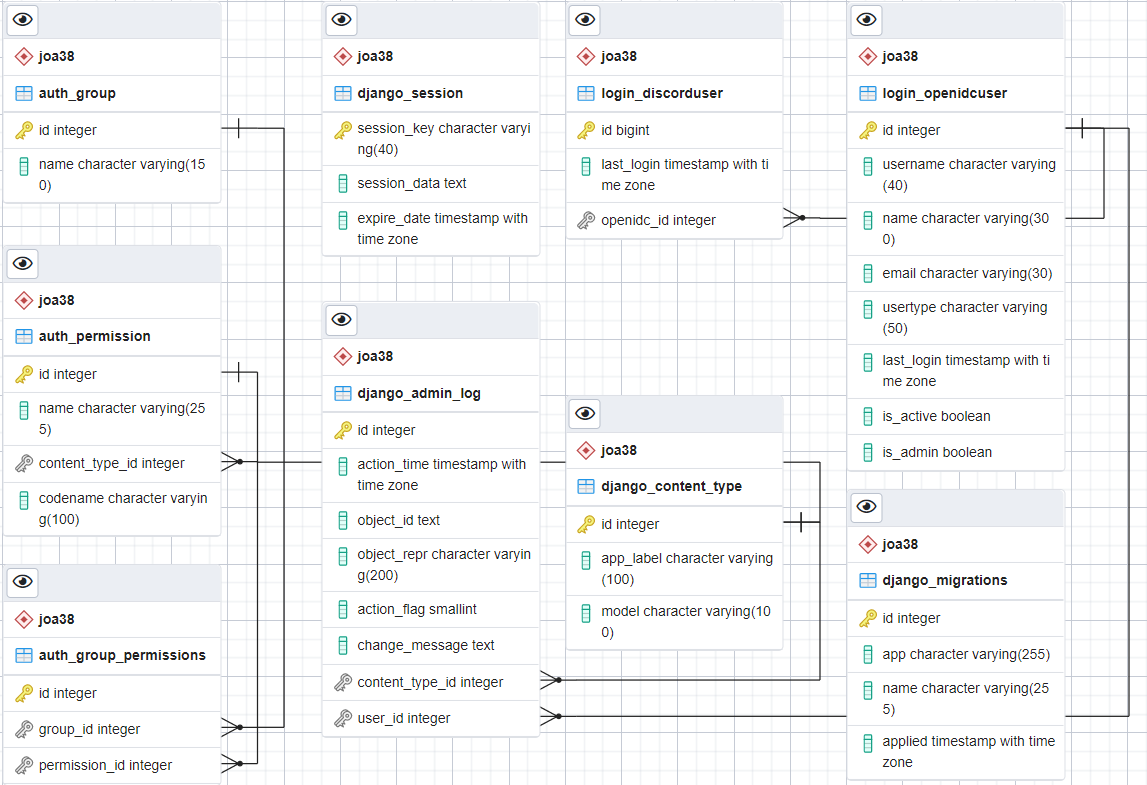
\includegraphics[width=1\linewidth]{Figures/er-diagram.png}
	\caption{Final Entity Relationship diagram for database}
	\label{fig:final-database}
\end{figure}

\begin{itemize}
	\item \textbf{User tables} - These two tables are the ones that have been discussed previously in this document for storing user data.
	\begin{itemize}
		\item \textbf{login\_openidcuser} - This table stores the OpenID Connect \cite{OpenID} information and is used as the authenticated user account.
		\item \textbf{login\_discorduser} - This table stores information on the discord user and contains a foreign key relationship with the table above.
	\end{itemize}
	\item \textbf{Django tables} - Tables generated by Django \cite{Django}
	\begin{itemize}
		\item \textbf{django\_migrations} - This table contains the history of the changes made to the database using Django. It acts as a way to revert to previous versions of the database in the case of 
		errors.
		\item \textbf{django\_session} - Stores sessions on the currently logged in users.
		\item \textbf{django\_content\_type} - Stores information on all available models in the database.
		\item \textbf{django\_admin\_log} - Stores history of logins for administrative users.
		\item \textbf{auth\_group \& auth\_group\_permissions \& auth\_permissions} - These tables are part of the backend for the authentication of users.
	\end{itemize}
\end{itemize}

Below are examples of the records that are stored in the database tables. 

\textbf{Note}: The column last\_login in the table \ref{tab:aber-table} contains the word datetime but should have a datetime object as seen in table \ref{tab:dis-table}. It has been removed so that the table fits nicely in this document.

\begin{table}[H]
	\centering
	\small
	\setlength\tabcolsep{2pt}
	\begin{tabular}{|c|c|c|c|c|c|c|c|}
		\hline
		\underline{id} & username & name & email & usertype & last\_login & is\_active & is\_admin \\
		\hline
		1 & joa38 & Joel Adams & joa38@aber.ac.uk & staff & datetime & t & t \\
		2 & jet39 & Jenny Thyer & jet39@aber.ac.uk & student & datetime & t & f \\
		3 & maw86 & Michael Antony West & maw86@aber.ac.uk & student & datetime & t & f \\
		\hline 
	\end{tabular}
	\caption{Aberystwyth user table example}
	\label{tab:aber-table}
\end{table}

\begin{table}[H]
	\centering
	\small
	\setlength\tabcolsep{2pt}
	\begin{tabular}{|c|c|c|}
		\hline
		\underline{id}                 & last\_login                   & openidc\_id* \\
		\hline
		727834884915331144 & 2021-02-18 16:43:47.067328+00 & 1           \\
		284352754321719296 & 2021-02-18 16:43:47.067328+00 & 1           \\
		246998944964542464 & 2021-02-04 11:14:40.057891+00 & 2           \\
		282248714955784192 & 2021-02-12 17:35:23.044226+00 & 3           \\
		\hline
	\end{tabular}
	\caption{Discord user table example}
	\label{tab:dis-table}
\end{table}

\section{Configuration and Setup}
After completion of this project there is a plan to setup this service permanently for the department so I have created a folder called \textit{config} containing information on how to set up this project. This folder contains a README.md file that explains how and what is needed to be configured to get the system up and running properly. I have also added a bash script called setup.sh that installs and the relevant dependencies and sets up the virtual environments for the projects. Also included are a few example configuration files for Apache2 \cite{apache2}, Django \cite{Django}, OpenID Connect authentication \cite{OpenID} and Discord.py \cite{discord.py}.

\section{Unforeseen Issues}\label{sec3:unforeseen}
An issue that I encountered was with creating the custom user model in Django that would have been used to model the database. The documentation and videos I found online about implementing user models were rather cryptic and difficult to understand, however I eventually found a video explaining how to implement a good custom user model. Once this was completed I realised that Django isn't happy with modelling the primary key of a table using a char so I had to switch to using an int. This turned out to be a good idea as Aberystwyth university tends to recycle old emails so over the next 5 years there could be an issue where the database would try and create a new entry in the database with the same email.
\begin{figure}[H]
	\centering
	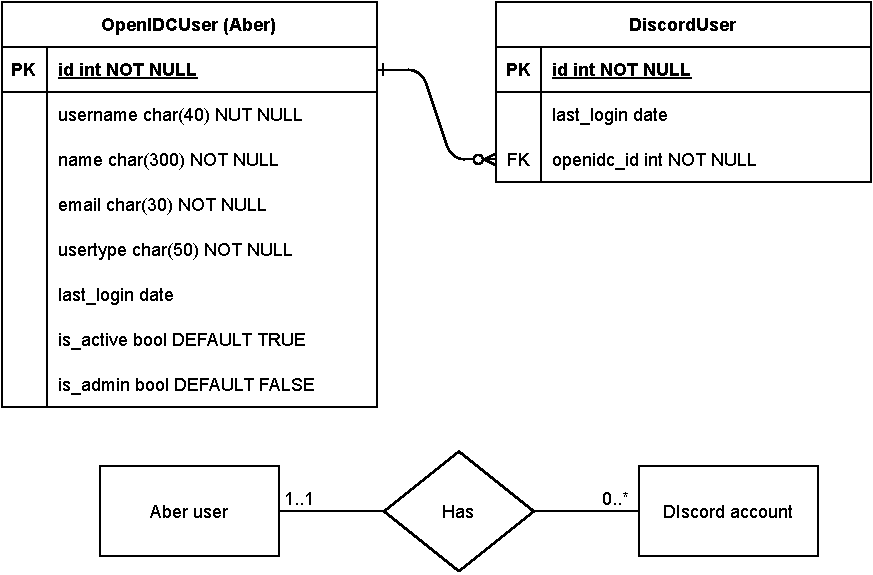
\includegraphics[width=0.8\linewidth]{Figures/database-er-1}
	\caption{Updated Entity relationship diagram for database}
	\label{fig:database-er-1}
\end{figure}

\section{Review}
\subsection{Review Against Planned Requirements}\label{sec3:pr}
Most of the planned requirements haven't changed during implementation however some of the promised tasks have only been partially fulfilled. Please see Appendix \ref{tab:fr-test} for a table of the functional requirements specified in \ref{sec1:fr}. For more information on requirements that did not pass please see \ref{sec4:fr}.

In the final section of section \ref{sec1:obj} \textbf{Further potential work} I have decided against integrating DemoHelper into AberLink as this would greatly increase it's complexity and make it much more difficult to maintain. I have also not added Welsh language support as I do not speak the language fluently nor understand it.

\subsection{Review Against Project Process}\label{sec3:pp}

Below is included a table describing the iterations and what was completed each one. These iterations were based on the list of objectives created in section \ref{sec1:obj} and span over the course of two months. For more detail please see the wordpress blog here \href{https://cs39440blog.wordpress.com/}{https://cs39440blog.wordpress.com/}.

\begin{longtable}[H]{| c | c | p{9cm} |}
\hline
Iteration & Time taken (days) & What happened? \\
\hline
1 & 5 & Research into services required to run the project and basic setup of uni container. Lots of meetings to discuss what data I can use and began setup of API endpoint for attendance. \\
\hline
2 & 5 & Setup HTTPS on container, installed Django \cite{Django} and created basic website using it. Linked up Django to database and created basic Discord login system. \\
\hline
3 & 5 & Added OpenID Connect \cite{OpenID} to website for aber user login. Created basic models to link OpenID accounts to Discord accounts in PostgreSQL \cite{psql}. \\
\hline
4 & 7 & Created Admin pages and implemented proper database model for Discord and Aber users\\
\hline
5 & 5 & Created Discord bot skeleton and added support for it to connect to the database.\\
\hline
6 & 5 & Added attendance and verification to Discord bot. \\
\hline
7 & 5 & Added content to main webpage and option to delete a Discord account or all data. Added custom error message webpages for 400, 403, 404 and 500. \\
\hline
8 & 5 & Updated main user page so that it queries Discord API to get profile picture and username and update webpage with details. Added more features to Discord bot to interact with database.\\
\hline
9 & 5 & Created Configuration folder for installing the software along with bash script to install dependencies.\\
\hline
10 & 5 & Added Discord bot functionality to add configurations to a server and feature to automatically change Discord users nickname to append aber email.\\
\hline
11 & 16 & Working on LaTeX document for project report. \\
\hline
\caption{Project iterations and what occurred}
\label{tab:project-iterations}
\end{longtable}

I've included a graph below of my GitLab commits over time below to help backup my table described above. 

\begin{figure}[H]
	\centering
	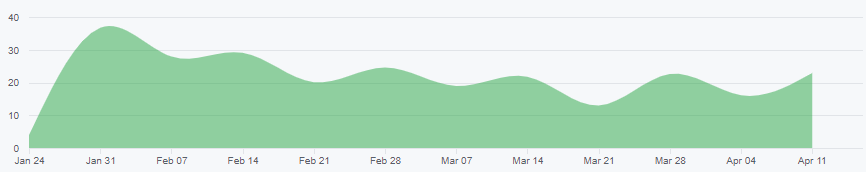
\includegraphics[width=1\linewidth]{Figures/gitlab-commit-graph.png}
	\caption{GitLab graph of commits over time}
	\label{fig:gitlab-graph}
\end{figure}